\chapter{Measuring distance to wall}
\label{chap:wall_dist}

\section{Practical use of }
%How we inplemented it to solving obstacles around the track.
%Why do we use two of them?
On the track is a variety of different obstacles and some of them require informations about distance. To solve these tasks the robot needs a devise to measuring distance. 

The two obstacle where the IR sensors is used:
\begin{itemize}
\item Obstacle 1: Go to the wall stop 20cm from the wall turn and return to the line.
\item Obstacle 2: Go around the corner and stop on the cross.
\end{itemize}

\section{IR sensor}
The IR sensors that is used is the SHARP 2d120x which is a nonlinear devise. The IR sensor works by sending a infrared beam out, the beam then returns  back to the device after hitting a surface or a obstacle, the angle that the beam returns with determines the distance. 
  \begin{figure}[!h!]
	\centering
	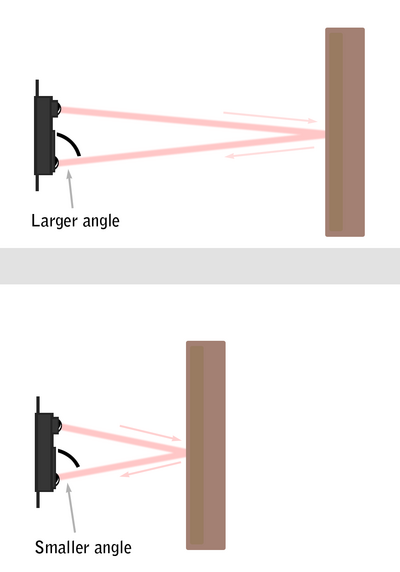
\includegraphics[width=0.15\textwidth]{irsensor.png}
	\caption{Distance IR sensor}
	\label{fig:3}
\end{figure}




\section{Converting using an ADC}
The IR sensor returns a voltage value that is converted in to a unsigned binary one byte number in the MCU's ADC (Analog to Digital Converter) but because of the nonlinearity in the device a equation is made by plotting measurements from 1cm to 50cm. A best fitting trend line it made and from that a equation is used with the output from the ADC to give the distance in cm.
  \begin{figure}[!h!]
	\centering
	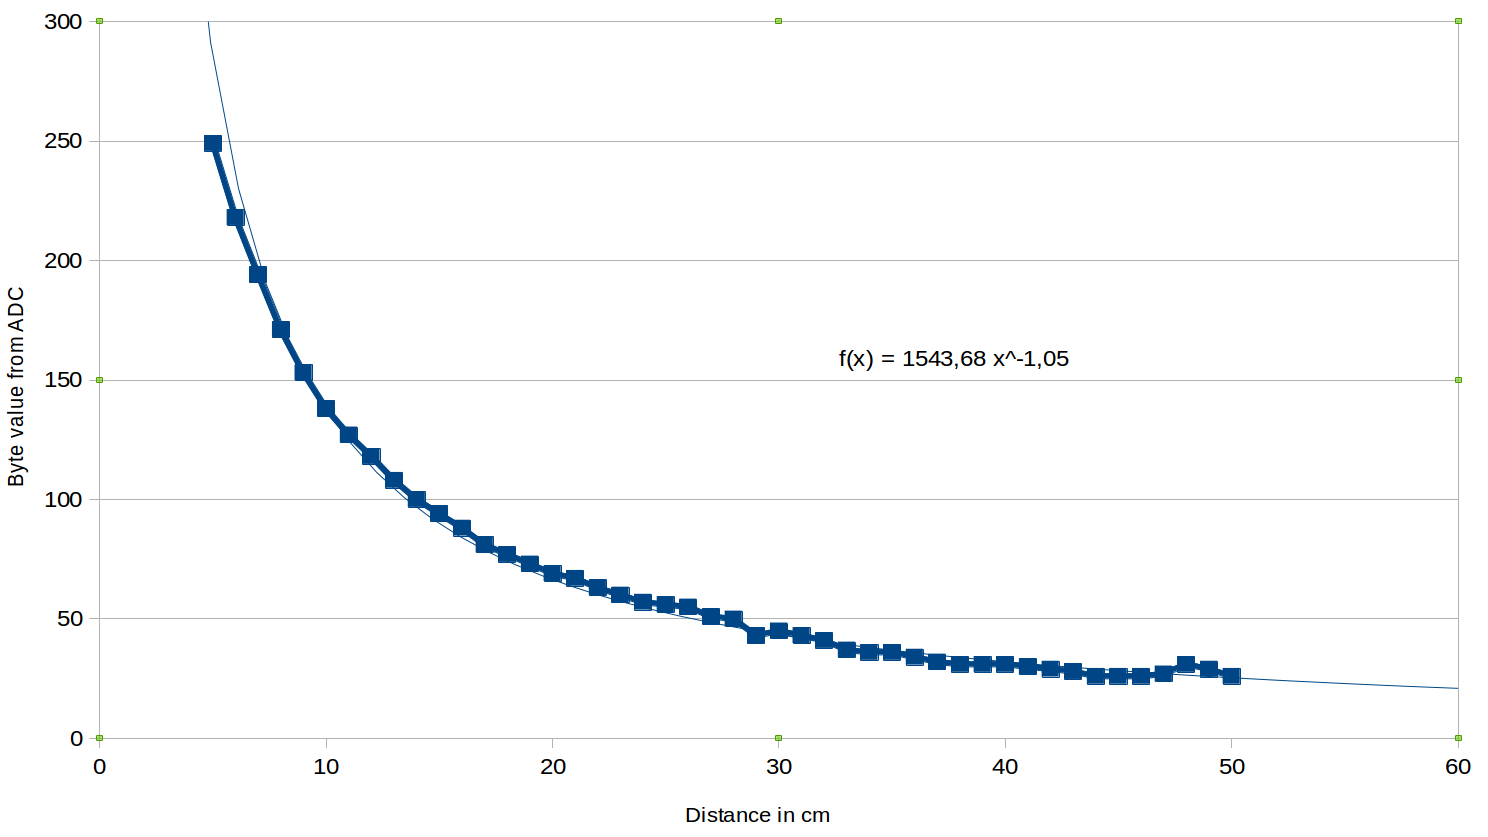
\includegraphics[width=0.9\textwidth]{adcgraf.png}
	\caption{Distance IR sensor}
	\label{fig:3}
\end{figure}

The equations is then fund to by:

\begin{equation}
f(x) = 1543.68^{-1.0.5}
\end{equation}




